% !TEX root =  ../main_manuscript.tex 
\section{Results}
The cause-specific cumulative upgrading-risk at year five of follow-up was 35\% in PRIAS, and at most 50\% in the six validation cohorts (Panel~B, Figure~\ref{fig:auc_beforecalib}). That is, many patients may not require all biopsies planned in the first five years of AS. In the PRIAS based fitted model, the adjusted hazard ratio (aHR) of upgrading for an increase in patient age from 61 to 71 years (25-th to 75-th percentile) was 1.45~(95\%CI:~1.30--1.63). For an increase in fitted PSA value (log scale) from 2.36 to 3.07 (25-th to 75-th percentile), the aHR was 0.99~(95\%CI:~0.89--1.11). The strongest predictor of upgrading-risk was instantaneous PSA velocity, with an increase from -0.09 to 0.31 (25-th to 75-th percentile), leading to an aHR of 2.47~(95\%CI:~1.93--2.99). The aHR for PSA value and velocity varied between cohorts (Table~8, Supplementary~A.2).

The time-dependent MAPE; time-dependent AUC; and calibration plot of our model in different validation cohorts are shown in Panel~B, Figure~8, Supplementary~B; Panel~A, Figure~\ref{fig:auc_beforecalib}; and Panel~B, Figure~\ref{fig:auc_beforecalib}, respectively. In all cohorts, time-dependent AUC was moderate (0.55 to 0.75) over the whole follow-up period. Time-dependent MAPE was large (0.3 to 0.45) in those cohorts where the impact of PSA value and velocity on upgrading-risk was different from PRIAS (e.g., MUSIC cohort, Table~8, Supplementary~A.2), and moderate (0.1 to 0.3) otherwise. In all cohorts, the MAPE decreased rapidly after year one of follow-up. Our model was miscalibrated for validation cohorts (Panel~B, Figure~\ref{fig:auc_beforecalib}). We resolved this by recalibrating the baseline hazard of upgrading in all cohorts (Figure~6, Supplementary~B). We compared risk predictions from the recalibrated models with predictions from separately fitted joint models to each cohort (Figure~7, Supplementary~B). The difference in predictions was lowest in Johns Hopkins cohort (impact of PSA similar to PRIAS, Table~5, Supplementary~A.2). Comprehensive results are in Supplementary~A.2~and~B.

\begin{figure}
\centerline{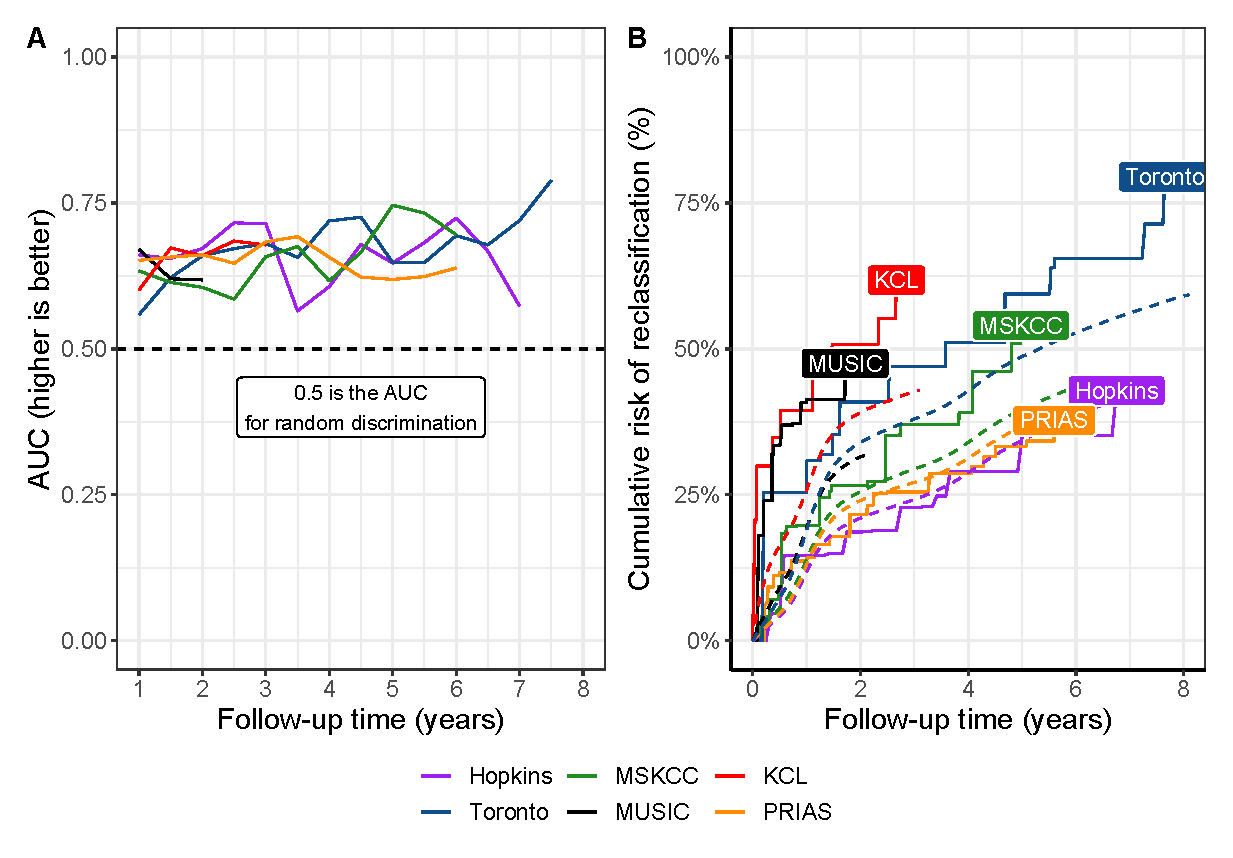
\includegraphics[width=\columnwidth]{images/auc_beforecalib.eps}}
\caption{\textbf{Model Validation Results}. \textbf{Panel~A}: time-dependent area under the receiver operating characteristic curve or AUC (measure of discrimination). \textbf{Panel~B}: calibration-at-large indicates model miscalibration. This is because solid lines depicting the non-parameteric estimate of the cause-specific cumulative upgrading-risk~\citep{turnbull1976empirical}, and dashed lines showing the average cause-specific cumulative upgrading-risk obtained using the joint model fitted to the PRIAS dataset, are not overlapping. Same plot after recalibration is shown in Figure~6, Supplementary~B. Full names of Cohorts are \textit{PRIAS}: Prostate Cancer International Active Surveillance, \textit{Toronto}: University of Toronto Active Surveillance, \textit{Hopkins}: Johns Hopkins Active Surveillance, \textit{MSKCC}: Memorial Sloan Kettering Cancer Center Active Surveillance, \textit{KCL}: King's College London Active Surveillance, \textit{MUSIC}: Michigan Urological Surgery Improvement Collaborative Active Surveillance, \textit{UCSF}: University of California San Francisco AS.}
\label{fig:auc_beforecalib}
\end{figure}

\subsection{Personalized Biopsy Schedules}
We utilized the PRIAS based model to create personalized biopsy schedules. Specifically, first, we utilized the model to predict a patient's cause-specific cumulative upgrading-risk on his future follow-up visits (usually every six months in PRIAS) based on his available data (Figure~\ref{fig:demo_pat1}). We then planned biopsies on those visits where the patient's conditional cumulative upgrading-risk was more than a certain threshold (Supplementary~C). Example personalized schedules based on 5\% and 10\% risk thresholds are shown in Figure~\ref{fig:demo_pat1}, and in Figure~9--11, Supplementary~C. For both personalized and fixed schedules, we estimated the expected time delay in detecting progression if a patient follows them (Panel~C, Figure~\ref{fig:demo_pat1}). The delay is calculated in a patient-specific manner (Supplementary~C) and is updated as more data becomes available over follow-up. Using expected delay and schedule of biopsies as criteria, patients/doctors can compare fixed schedules with personalized schedules based on different risk thresholds.

\begin{figure}
\centerline{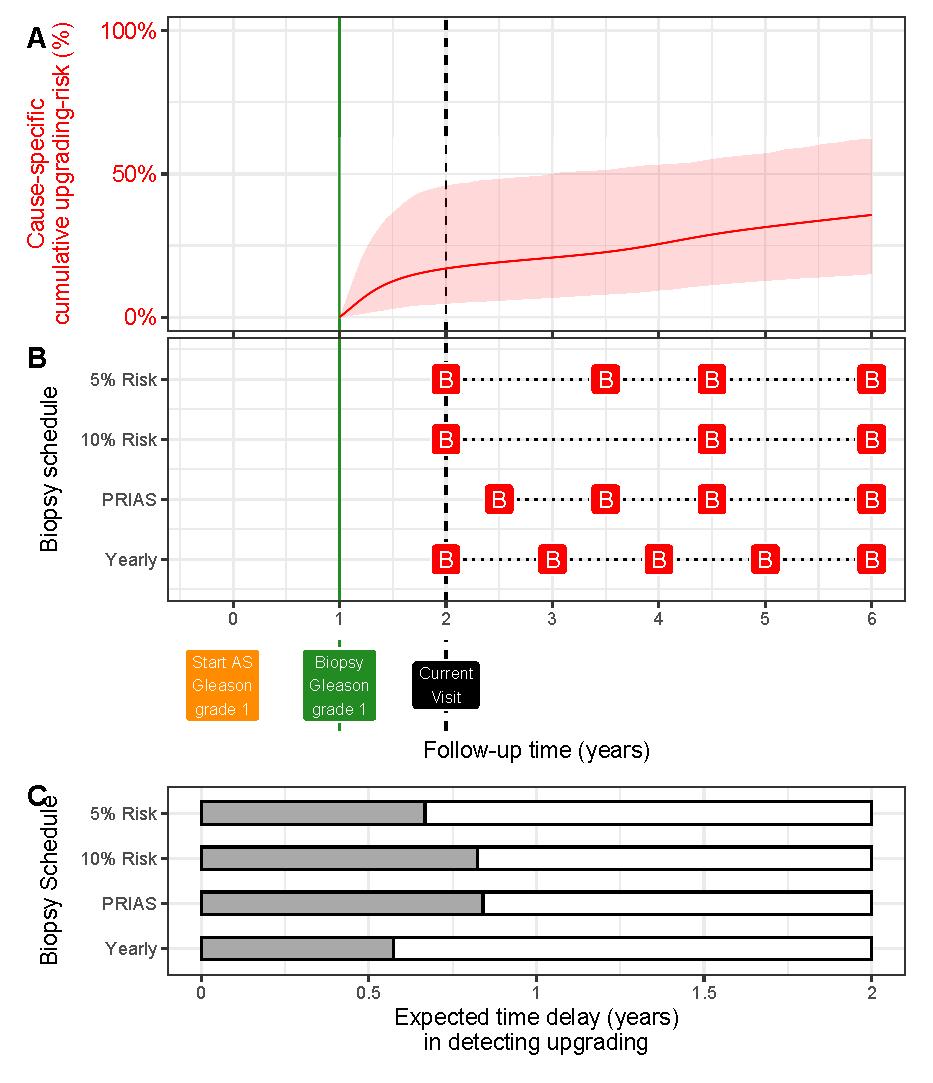
\includegraphics[width=\columnwidth]{images/demo_pat1.eps}}
\caption{\textbf{Illustration of personalized and fixed schedules of biopsies}. Due to a lack of space, the PSA profile of this patient is shown in Figure~\ref{fig:jmExplanationPlot_113}. \textbf{Panel~A:} Predicted cumulative upgrading-risk (95\% credible interval shaded). \textbf{Panel~B:} Personalized and fixed schedules of biopsies, with a red `B' indicating a scheduled biopsy. The green vertical line at year 1 denotes the time of the latest negative biopsy. Black dashed line at year 3 denotes the time of the current visit. \textbf{Panel~C:}\ Expected time delay in detecting upgrading (months) for different schedules. A compulsory biopsy was scheduled at year six (maximum biopsy scheduling time in PRIAS, Supplementary~C) in all schedules for a meaningful comparison between them.}
\label{fig:demo_pat1}
\end{figure}

\subsection{Web-Application}
We implemented our model and personalized schedules in a user-friendly web-application \url{https://emcbiostatistics.shinyapps.io/prias_biopsy_recommender/}. Currently, the web-application supports PRIAS and the six validation cohorts. Patient data can be entered manually and in Microsoft Excel format. Predictions for upgrading-risk are available for a currently limited, cohort-specific, follow-up period (Table 7, Supplementary~C). The web-application visualizes the timing of biopsies, and expected time delay in detecting upgrading, for personalized schedules based on 5\%, 10\%, and 15\% risk threshold; annual biopsies; biennial biopsies; and PRIAS schedule.